\chapter{TINJAUAN PUSTAKA}
		\section{Python}
        		Python adalah bahasa pemrograman interpretatif, interaktfi dan berorientasi objek. Python menggabungkan modul, pengecualian, penulisan secara dinamis, tipe data dinamis yang sangat tinggi dan kelas. Python memiliki antarmuka ke banyak \textit{system call} dan pusataka diberbagai sistem dan dapat diperluas ke bahasa pemrograman C atau C++. Python dapat berjalan pada berbagai sistem operasi seperti Unix, Linux, Mac Os dan Windows.\\
                \indent Python adalah bahasa pemrograman tingkat tinggi yang dapat diterapkan pada berbagai masalah. Bahasa ini dilengkapi pustaka yang besar untuk melakukan pemrosesan \textit{string}, protokol internet, rekayasa perangkat lunak dan antarmuka sistem operasi\cite{python_faq}.\\
                \indent Dilihat dari kelebihan, bahasa pemrograman Python dapat digunakan dalam pengembangan aplikasi yang kompleks. Pada tugas akhir ini, bahasa pemrograman Python digunakan untuk pembuatan \textit{middleware}.
        \section{Flask}
         	Flask adalah kerangka aplikasi web Python yang ringan. Flask dirancang untuk memulai membuat web dengan cepat dan mudah, dengan kemampuan untuk membuat aplikasi web sampai tingkat yang rumit. Flask dibuat dengan terintegrasi dengan modul Werkzeug dan Jinja. Flask termasuk salah satu kerangka aplikasi web Python yang populer.\\
            \indent Flask didesain tidak memiliki depedensi dan tata letak kerangka aplikasi, dengan demikian pengembang memiliki kebebasan untuk mengatur kerangka aplikasinya sendiri serta menambahkan modul yang diperlukan sesuai kebutuhan. Flask memiliki berbagai ekstensi yang dikembangkan oleh komunitas sehingga dapat menambahkan berbagai fungsi dengan mudah\cite{about_flask}. \\
            \indent Flask memiliki kelebihan yaitu sangat ringan dan sangat sederhana dalam proses pengembangan. Sehingga Flask sangat cocok digunakan untuk pembuatan \textit{HTTP Rest API}. Pada tugas akhir ini, Flask akan digunakan untuk pembuatan \textit{HTTP Rest API}. \\
            \indent Pada tugas akhir ini FLask akan digunakan untuk mengatur end-point yang digunakan sistem untuk menerjemahkan perintah dari pengguna sistem.
        
       	\section{Gitpython}
            Gitpython adalah pustaka python untuk berinteraksi dengan repositori git, dalam interaksi level tinggi seperi git-porcelain maupun level rendah seperti git-plumbing.\\ 
            \indent Gitpython menyediakan konsep dari obyek git untuk mempermudah mengakses data repositori dan juga mampu untuk mengakses repositori git secara langsung baik dengan implementasi python atau dengan menggunkan commnand git.\cite{about_gitpython} \\
            \indent Pada tugas ini gitpython akan digunakan melakukan eksekusi perintah git yang akan digunakan oleh sistem dalam mengatur pelacakan konfigurasi perangkat jaringan.\\
            
        \section{Python Watchdog}
            Python watchdog adalah modul dari python untuk mengawasi \textit{event} dari suatu file system .Watchdog dapat menangkap semua operasi yang terjadi di dalam direktori yang di tentukan.Watchdog bekerja secara real time dengan menggunakan thread.\cite{watchdog_python} \\     
            \indent Pada tugas akhir ini python watchdog akan digunakan untuk melihat perubahan yang terjadi pada file konfigurasi perangkat jaringan yang disimpan oleh sistem.\\
        
        \section{TFTP}
        	Trivial File Transfer Protocol (TFTP) adalah protokol pengiriman file yang sederhana tanpa menggunakan autentikasi pengguna. TFTP menggunakan protokol UDP dalam pengiriman data. TFTP tidak bisa digunakan untuk melihat isi dari suatu direktori, TFTP hanya bisa digunakan untuk mengirim dan menerima data.\cite{tftp}\\
        	\indent Dalam tugas akhir ini TFTP akan digunakan untuk jalur pengiriman file konfigurasi perangkat jaringan yang menggunakan protokol TFTP.
        	
        \section{FTP}
        	File Transfer Protocol (FTP) adalah protokol untuk mengirim file dari \textit{server} ke \textit{client} dengan menggunakan model \textit{client-server}. FTP menggunakan protokol TCP dalam pengiriman \textit{file}. FTP memiliki dua mode yaitu mode pasif dan mode aktif yang menentukan bagaiman client dan server terhubung.\cite{ftp}\\
        	\indent Dalam tugas akhir ini FTP akan digunakan untuk menerima konfigurasi yang dikirim oleh perangkat jaringan melalui protokol FTP.
        	
       	\section{Git}
       		Git merupakan salah satu jenis dari VCS (\textit{Version Control System}) yang banyak digunakan oleh pengembang aplikasi saat ini. Git merupakan VCS yang gratis dan sumber terbuka. Git didesain untuk menangani proyek dari yang sederhana hingga yang kompleks dengan kecepatan dan efisiensi yang baik\cite{git_about}. Git memiliki dua jenis \textit{repository} yakni \textit{local repository} dan \textit{remote repository}. \textit{Local repository} merupakan \textit{repository} yang berada pada komputer kita dan \textit{remote repository} adalah \textit{repository} yang berada di server lain yang juga terhubung dengan \textit{local repository} sehingga data yang ada pasti sama.
       		
       			\begin{figure}[H]
       			\centering
       			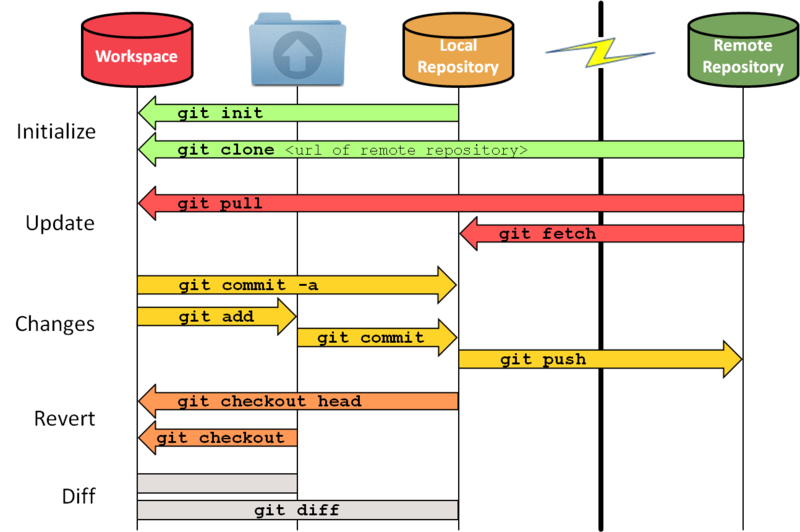
\includegraphics[width=\textwidth]{Images/C-2/Git_workflow.png}
       			\caption{alur kerja git \cite{git_workflow} }
       			\label{GitWorkflow}
       			\end{figure}
       		
        	
        
